\documentclass[a4paper,10pt]{scrreprt}

\usepackage[ngerman]{babel}
\usepackage[utf8]{inputenc} 
\usepackage{lmodern}
\usepackage{listings}
\usepackage{color}
\usepackage{amsmath}
\usepackage{amssymb}
\usepackage{pdfpages}
\usepackage{geometry}
\usepackage{fancyhdr}


\pagestyle{fancy}
\lhead{}
\chead{Protokoll zum Praktikum Programmierbare Schaltkreise}
\rhead{}
\lfoot{Christian Kroh \texttt{(s1428123)}}
\cfoot{\thepage}
\rfoot{Patrick Russell \texttt{(sxxx)}}

\geometry{a4paper,left=2cm,right=2.5cm, top=1.5cm, bottom=2cm} 


\lstset{%
    columns=fullflexible,
    aboveskip=5pt,
    belowskip=10pt,
    basicstyle=\small\ttfamily,
    numbers=left,
    stepnumber=1, 
    numbersep=13pt,
    showspaces=false,
    showstringspaces=false,
    showtabs=false,
    xleftmargin=20pt,
    xrightmargin=10pt,
    framesep=5pt,
    framerule=3pt,
    frame=leftline,
    tabsize=2,
    breaklines=true,
    breakatwhitespace=true,
}


\renewcommand{\thechapter}{\hspace*{-1.0em}}
\renewcommand{\thesection}{\hspace*{-1.0em}}
\renewcommand{\thesubsection}{\arabic{section}.\arabic{subsection}}

\title{Protokoll zum Praktikum Programmierbare Schaltkreise}
\subtitle{Fakultät Informatik\\TU Dresden}

\author{
	\textbf{Christian Kroh}\\ 
	\texttt{Matrikelnummer: 3755154} \\ \texttt{Studiengang: Informatik (Diplom)} \\ \texttt{Jahrgang: 2010/2011}
	\and
	\textbf{Patrick Russell}\\
	\texttt{Matrikelnummer: xxx} \\ \texttt{Studiengang: Informatik (Diplom)} \\ \texttt{Jahrgang: 2010/2011}
}

\date{\today{}, Dresden}



\begin{document}

\maketitle
			
\newpage
\section{Aufgabe 1 - Binär-Dekoder}
\subsection{Entwurf}
\begin{description}
	\item[Input] 4-Bit Binärzahl durch Schieberegister SW3 ... SW0
	\item[Output] 7-Segmente Darstellung einer Hexadezimalziffer (8 Einzelsignale = 7 Segmente + 1 Punkt)
\end{description}

\begin{tabular}{|c|c|c|c||c|c|c|c|c|c|c|c|c|}
\hline
\multicolumn{4}{|c|}{Input} & \multicolumn{9}{|c|}{Output} \\
\hline
\textsc{SW3} & \textsc{SW2} & \textsc{SW1} & \textsc{SW0} & 
\textsc{Hex} & \textsc{A} & \textsc{B} & \textsc{C} & \textsc{D} & \textsc{E} & \textsc{F} & \textsc{G} & \textsc{dot} \\ 
\hline
\hline
0 & 0 & 0 & 0 & 0 & 0 & 0 & 0 & 0 & 0 & 0 & 1 & 1 \\ 
0 & 0 & 0 & 1 & 1 & 1 & 0 & 0 & 1 & 1 & 1 & 1 & 1 \\
0 & 0 & 1 & 0 & 2 & 0 & 0 & 1 & 0 & 0 & 1 & 0 & 1 \\
0 & 0 & 1 & 1 & 3 & 0 & 0 & 0 & 0 & 1 & 1 & 0 & 1 \\
0 & 1 & 0 & 0 & 4 & 1 & 0 & 0 & 1 & 1 & 0 & 0 & 1 \\
0 & 1 & 0 & 1 & 5 & 0 & 1 & 0 & 0 & 1 & 0 & 0 & 1 \\
0 & 1 & 1 & 0 & 6 & 0 & 1 & 0 & 0 & 0 & 0 & 0 & 1 \\
0 & 1 & 1 & 1 & 7 & 0 & 0 & 0 & 1 & 1 & 1 & 1 & 1 \\
1 & 0 & 0 & 0 & 8 & 0 & 0 & 0 & 0 & 0 & 0 & 0 & 1 \\
1 & 0 & 0 & 1 & 9 & 0 & 0 & 0 & 0 & 1 & 0 & 0 & 1 \\
1 & 0 & 1 & 0 & A & 0 & 0 & 0 & 1 & 0 & 0 & 0 & 1 \\
1 & 0 & 1 & 1 & b & 1 & 1 & 0 & 0 & 0 & 0 & 0 & 1 \\
1 & 1 & 0 & 0 & C & 0 & 1 & 1 & 0 & 0 & 0 & 1 & 1 \\
1 & 1 & 0 & 1 & d & 1 & 0 & 0 & 0 & 0 & 1 & 0 & 1 \\
1 & 1 & 1 & 0 & E & 0 & 1 & 1 & 0 & 0 & 0 & 0 & 1 \\
1 & 1 & 1 & 1 & F & 0 & 1 & 1 & 1 & 0 & 0 & 0 & 1 \\
\hline
\end{tabular}			
			
\subsection{Auswertung}
\begin{description}
\item[Ressourcenbedarf] 7 Logik-Elemente und 12 Pins
\end{description}

	
\newpage
\section{Aufgabe 2 - Hamming-Distanz}
\subsection{Entwurf}
\begin{description}
	\item[Input] 2 4-Bit Werte 
		\begin{itemize}
			\item 1.Wert: 4-Bit Binärzahl durch Schieberegister SW3 ... SW0
			\item 2.Wert: 4-Bit Binärzahl durch Schieberegister SW7 ... SW4
		\end{itemize}
	\item[Output] 7-Segmente Darstellung einer Hexadezimalziffer (8 Einzelsignale = 7 Segmente + 1 Punkt)
	\item[Ansatz] SW3 ... SW0 und SW7 ... SW4 logisch xor verknüpfen und Ergebnis direkt auf 7-Segmente Anzeige mappen
\end{description}	
(\ref{lst:02-hamming}~Hamming.vhdl Code)

\subsection{Auswertung}
\paragraph{Ressourcenbedarf}
\begin{itemize} 
\item 9 Logik-Elemente
\item 16 Pins 
\end{itemize}

	
\newpage
\section{Aufgabe 3 - Modulo-n-Zähler}
\subsection{Entwurf}
\begin{description}
\item[a)] Der Zähler ist nach 50 Millionen Schritten zurückzusetzen (50 MHz Takt entspricht 50 Millionen Taktperioden pro Sekunde)
\item[b)] Für das Schieberegister ist der Zählerzustand ein Enable-Signal
\item[c)] \hfill 
	\begin{description}
	\item[Input] \hfill 
		\begin{itemize}
			\item 50MHz Takt
			\item Reset (Schiebeschalter SW0)
		\end{itemize}
	\item[Output] LED-Zeile
	\item[Ansatz] 2 Komponenten: Schieber und Zähler 
	\end{description}	
\end{description}
\paragraph{Zähler} gibt alle 50-Millionen Taktperioden (50MHz Takt ergibt $50\cdot10^6$ Taktschritte pro Sekunde) einen Takt lang ein enable-Signal aus. 
(\ref{lst:03-zaehler}~Zaehler.vhdl-Code)
\paragraph{Schieber} beinhaltet den Zähler als Komponente und verschiebt bei dessen enable-Signal die LED-Anzeige um eine Stelle pro Takt. (\ref{lst:03-schieber}~Schieber.vhdl-Code)

\subsection{Auswertung}
\paragraph{Ressourcenbedarf}
\begin{itemize} 
\item 60 Logik-Elemente
\item davon 38 dedizierte Logik-Elemente
\item 12 Pins 
\item maximale Taktfrequenz von 250 MHz
\end{itemize}

	
\newpage
\section{Aufgabe 4 - Entprell-Automat}
\subsection{Entwurf}
	\paragraph{State-Machine-Charts}\hfill \\

	\paragraph{LED} enthält die Komponente Entprellung und verbindet die Ein- und Ausgangssignale. (\ref{lst:04-led}~LED.vhdl-Code) \\
	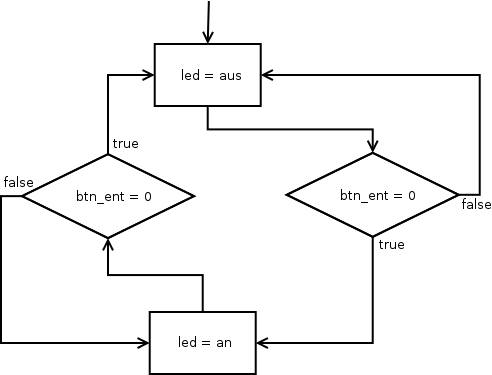
\includegraphics[width=0.7\textwidth]{resources/04-led.png}
	
	\paragraph{Entprellung} enthält die Komponente Zaehler, der bei der Veränderung des Eingangsignals gestartet wird und für 3ms weitere Änderungen ignoriert. (\ref{lst:04-entprellung}~Entprellung.vhdl-Code) \\
	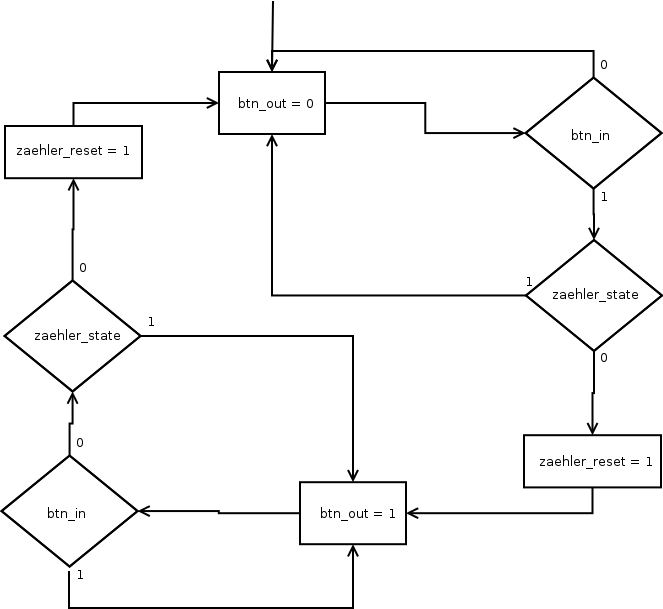
\includegraphics[width=0.8\textwidth]{resources/04-entpreller.png}


	\paragraph{Zaehler} implementiert einen Zähler, der durch ein Signal definierte Schritte zählt. Ausgegeben wird der aktuelle Zustand des Zählers. Eingegeben ein Reset-Signal. (\ref{lst:04-zaehler}~Zaehler.vhdl-Code) 
	\paragraph{Kopplung} \hfill\\
	Es wird eine synchrone Automatenkopplung über die Ausgangssignale mit einem Taktsignal verwendet.


\subsection{Auswertung}
	\paragraph{Ressourcenbedarf}
	\begin{itemize} 
	\item 86 Logik-Elemente
	\item davon 79 dedizierte Logik-Elemente
	\item 44 Register
	\item 3 Pins 
	\item maximale Taktfrequenz von 178 MHz
	\end{itemize}

	
\newpage
\section{Aufgabe 5 - HALLO-Anzeige}
\subsection{Entwurf}
	\begin{description}
	\item[zu a)] Es müssen 5 Zeichen kodiert werden (H, A, L, O, Leerzeichen).\\
			\\\(ld\, 5 = 3\)\\\\
			Daher werden für eine Binärkodierung mindestens 3 Bits benötigt.\\\\
			\begin{tabular}{|c|c|c||c|c|c|c|c|c|c|c|c|}
		\hline
		\multicolumn{3}{|c||}{Input} & \multicolumn{9}{|c|}{Output} \\
		\hline
		\textsc{BIT2} & \textsc{BIT1} & \textsc{BIT0} & 
		\textsc{CHAR} & \textsc{A} & \textsc{B} & \textsc{C} & \textsc{D} & \textsc{E} & \textsc{F} & \textsc{G} & \textsc{dot} \\ 
		\hline
		\hline
		0 & 0 & 0 &   & 1 & 1 & 1 & 1 & 1 & 1 & 1 & 1 \\ 
		0 & 0 & 1 & H & 1 & 0 & 0 & 1 & 0 & 0 & 0 & 1 \\
		0 & 1 & 0 & A & 0 & 0 & 0 & 1 & 0 & 0 & 0 & 1 \\
		0 & 1 & 1 & L & 1 & 1 & 1 & 0 & 0 & 0 & 1 & 1 \\
		1 & 0 & 0 & O & 0 & 0 & 0 & 0 & 0 & 0 & 1 & 1 \\
		\hline
	\end{tabular}
	\item[b)] Für das Schieberegister ist der Zählerzustand ein Enable-Signal
	\item[c)]
	\end{description}

	

\subsection{Auswertung}
	\paragraph{Ressourcenbedarf}
	\begin{itemize} 
	\item 73 Logik-Elemente
	\item 61 Register
	\item 34 Pins 
	\item maximale Taktfrequenz von 262 MHz
	\end{itemize}

	
\newpage
\section{Aufgabe 6 - Stoppuhr}
\subsection{Entwurf}
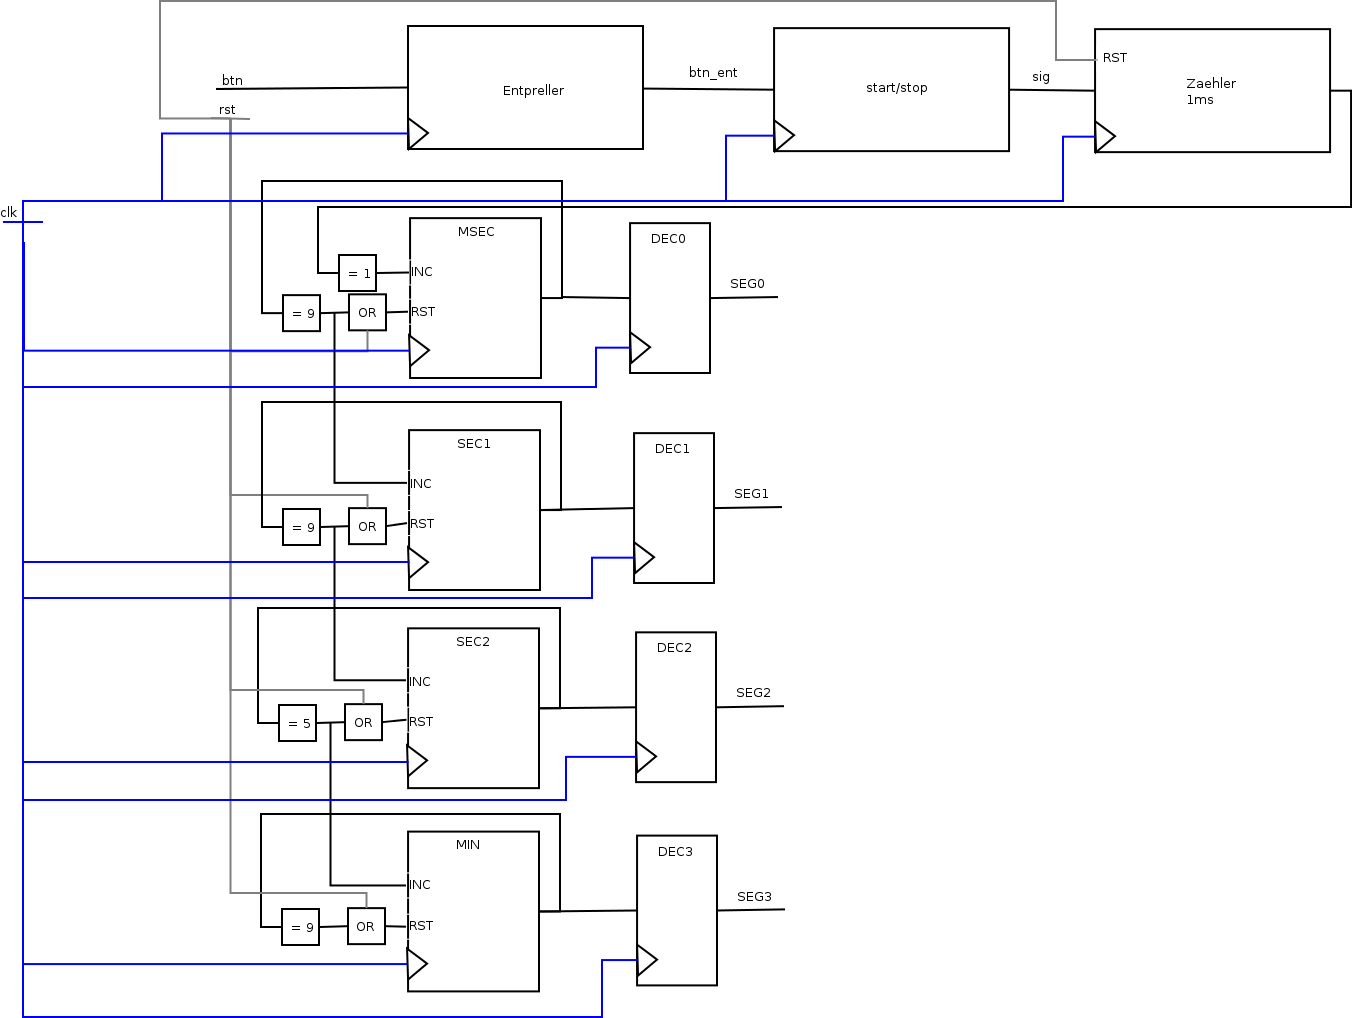
\includegraphics[width=1\textwidth]{resources/06-stopuhr.png}
	\newpage
	\paragraph{State-Machine-Charts}\hfill \\

		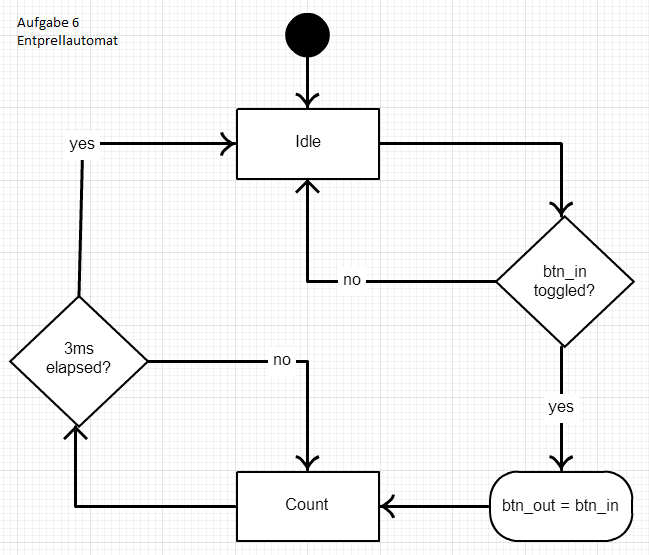
\includegraphics[width=0.8\textwidth]{resources/06-Entprellautomat.png}
		

		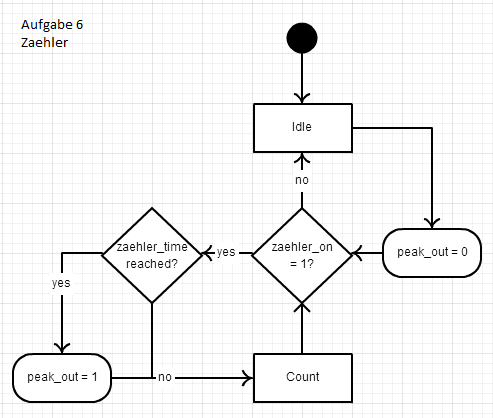
\includegraphics[width=0.7\textwidth]{resources/06-Zaehler.png}

		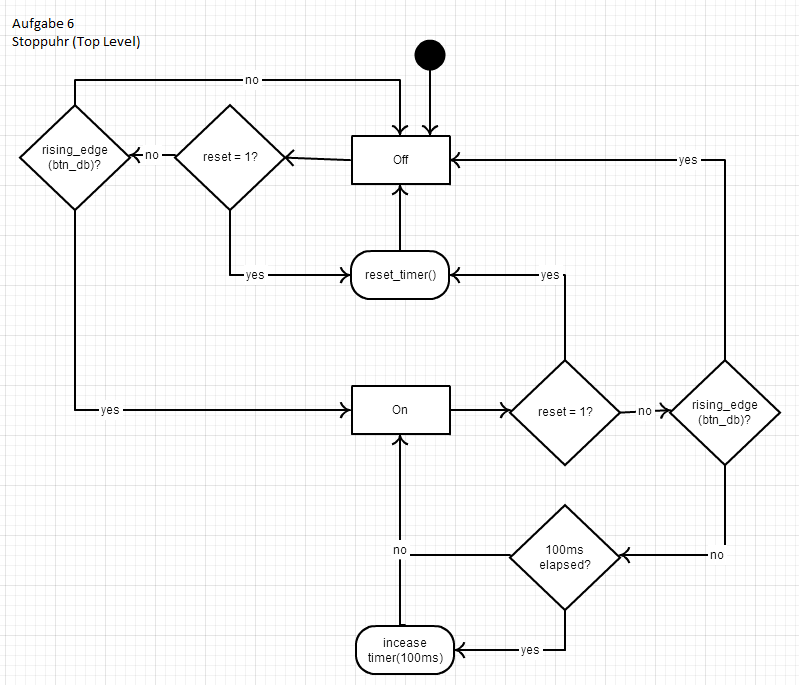
\includegraphics[width=0.7\textwidth]{resources/06-Stoppuhr.png}
 
\subsection{Auswertung}
	\paragraph{Ressourcenbedarf}
	\begin{itemize} 
	\item 163 Logik-Elemente
	\item davon 121 dedizierte Logik-Elemente
	\item 35 Pins 
	\item maximale Taktfrequenz von 225 MHz
	\end{itemize}

	
\newpage
\section{Anhang}
\subsection{01-Aufgabe Code}
\lstinputlisting[caption={VHDL-Code Decoder}, tabsize=2, numbers=left, language=VHDL]{src/Aufgabe_1/Decoder.vhdl}

\subsection{02-Aufgabe Code}
\lstinputlisting[caption={VHDL-Code Hamming-Distanz}, tabsize=2, numbers=left, language=VHDL]{src/Aufgabe_2/Hamming.vhdl}


\end{document}
